\section{Implementacja agentów}
\label{sec:implementacjaAgentow} 

\par Agenci stanowią główny trzon decyzyjny systemu. To w nich znajduje się logika odpowiedzialna za podejmowanie decyzji, reagowanie na zmiany i obsługę komunikatów nadawanych przez innych. Podstawowymi założeniami systemów agentowych jest ich autonomiczność, zdolność do komunikacji oraz możliwość postrzegania i wpływania na środowisko. Aby spełnić te wymagania koniecznym były zapewnienie pewnych mechanizmów.

\par Podstawą działania agentów, jest ich umiejętność do postrzegania otoczenia. Odbywa się to przy użyciu \texttt{IEnvironmentSignal}. Każdy agent w systemie definiuje, jakie sygnały z otoczenia potrafi obsłużyć. Następnie serwisy działające w ramach aplikacji, w której żyje nasz agent przekazują mu te sygnały. Trafiają one do specjalnej kolejki, skąd zostaną później obsłużone.

\par Zdolność do działania przejawia się poprzez dostęp do funkcji sprzętowych z poziomu aplikacji. Dla przykładu, \emph{Navigation Agent} potrafi wykorzystać \texttt{INavigationService}, aby ten wyświetlił patrolowi drogę do wyznaczonego celu.

\par Wszystkie te cechy (sygnały, akcje, wiadomości) można zidentyfikować, jako jedną z tych pięciu kategorii: relacje\english{Relations}, aktywność\english{Activity}, indywidualność\english{Individuality}, czas\english{Time} i lokalizacja\english{Location}. Ich wykaz, miejsce występowania oraz kategoria zostały przedstawione w tabeli \ref{tab:agentsFeaturesCategorization}.

\begin{table}[H]
    \centering
    \begin{tabular}{|c|c|c|} 
     \hline
     Agent & Nazwa & Kategoria \\
     \hline
     \hline
     \emph{Patrol Agent} & Patrolowanie & Aktywność \\ 
     \hline
     \emph{Patrol Agent} & Przemieszczenie się & Aktywność \\ 
     \hline
     \emph{Patrol Agent} & Rozwiązywanie interwencji & Aktywność \\ 
     \hline
     \emph{Patrol Agent} & Udział w strzelaninie & Aktywność \\ 
     \hline
     \emph{Patrol Agent} & Stan: w trakcie patrolowania & Indywidualność \\ 
     \hline
     \emph{Patrol Agent} & Stan: W trakcie oczekiwania na rozkaz & Indywidualność \\ 
     \hline
     \emph{Patrol Agent} & Posiadany rozkaz & Indywidualność \\ 
     \hline
     \emph{Patrol Agent} & Obecna lokalizacja & Lokalizacja \\ 
     \hline
     \emph{Patrol Agent} & Oczekiwanie na wsparcie & Relacja \\ 
     \hline
     \emph{Patrol Agent} & Czas otrzymania ostatniego rozkazu & Czas \\ 
     \hline
     
     \emph{Navigation Agent} & Wyświetlanie trasy do celu & Aktywność \\ 
     \hline
     \emph{Navigation Agent} & Lokalizacja docelowa & Indywidualność \\ 
     \hline
     \emph{Navigation Agent} & Obecna lokalizacja & Lokalizacja \\
     \hline

     \emph{Gun Agent} & Stan: Czy wystrzelono z pistoletu & Indywidualność \\
     \hline

     \emph{HQ Agent} & Stany patroli & Relacja \\
     \hline
     \emph{HQ Agent} & Przypisanie patroli do dzielnicy & Relacja \\
     \hline
     \emph{HQ Agent} & Lokalizacje patroli & Lokalizacja \\
     \hline
     \emph{HQ Agent} & Dzielnice, w których znajdują się patrole & Lokalizacja \\
     \hline
     \emph{HQ Agent} & Ustawienia algorytmu decyzyjnego & Indywidualność \\
     \hline
     \emph{HQ Agent} & Wydanie rozkazu patrolowi & Aktywność \\
     \hline
     \emph{HQ Agent} & Czas trwania strzelaniny & Czas \\
     \hline
     \emph{HQ Agent} & Czas trwania incydentu & Czas \\
     \hline

     Wszyscy agenci & Rozpoczęcie działania & Aktywność \\ 
     \hline\
     Wszyscy agenci & Zakończenie działania & Aktywność \\ 
     \hline
    \end{tabular}
    \caption{Tabela identyfikacji cech w kontekście agentów.}
    \label{tab:agentsFeaturesCategorization}
\end{table}

\par Dodatkowo, w systemie można opisać cykl życia zmiennych kontekstowych w następujący sposób:
\begin{itemize}
    \item Lokalizacja - jest pobierana przez \emph{Navigation Agent}, następnie przekazywana do \emph{Patrol Agent}, który przekazuje ją do \emph{HQ Agent}. Ten decyduje o tym, czy posiada już nowszą wersję tej informacji, czy też nie. W zależności od tego ignoruje lub zachowuje daną informację. Dodatkowo informacja ta jest wzbogacana o kontekst związany z dzielnicą.
    \item Trasa do celu - jest pobierana przez \emph{Nabigation Agent}, który następnie zachowuje ją u siebie i wyświetla.
    \item Wystrzał - sygnał obserwowany przez \emph{Gun Agent}, następnie przekazywany do \emph{Patrol Agent} i kierowany dalej do \emph{HQ Agent}, który na jej podstawie ogłasza alarm i wysyła jednostki w ramach wsparcia.
    \item Rozpoczęcie interwencji - sygnał obserwowany przez \emph{Patrol Agent}, zachowywany i przekazywany do \emph{HQ Agent}.
    \item Zakończenie interwencji - sygnał obserwowany przez \emph{Patrol Agent}, zachowywany i przekazywany do \emph{HQ Agent}.
    \item Zakończenie strzelaniny - sygnał obserwowany przez \emph{Patrol Agent}, zachowywany i przekazywany do \emph{HQ Agent}. Jednostka główna musi zdecydować, czy komunikat, który otrzymała nie jest duplikatem, jako iż, w strzelaninie może brać więcej niż jeden patrol.
    \item Poziom niebezpieczeństwa dzielnicy - informacja na ten temat jest posiadana przez \emph{HQ Agent}, na podstawie której wydaje on rozkazy patrolowania i rozwiązywania incydentów.
\end{itemize}

\par Komunikacja między agentami odbywa się przy wykorzystaniu \emph{Message Bus}a., opisanego w podrozdziale \ref{sec:infrastrukturaKomunikacyjna}. Wszystkie wiadomości spełniają interfejs \texttt{IMessage}, a agenci definiują które ich typy są w stanie obsłużyć. Oczywiście sama możliwość wysłania komunikatu, nie rozwiązuje wszystkich problemów w dialogu, dlatego też zostały zaimplementowane dwa dodatkowe mechanizmy rozszerzające bazowe możliwości.

\par Pierwszym z nich jest możliwość odpytania\english{Ask} innego agenta i oczekiwania na odpowiedź. Jest to niezbędny mechanizm, podczas podejmowania decyzji wymagających danych, których dany agent nie posiada.

\par Drugim wysyłanie wiadomości wymagających potwierdzenia odbioru\english{Requiring Acknowledgment}. Dla nich powstał specjalny interfejs \texttt{IMessageWithAcknowledgeRequired} rozszerzający \texttt{IMessage}. Mechanizm ten jest wykorzystywany podczas wysyłania rozkazów przez \emph{HQ Agent}, aby mieć pewność ich akceptacji.

\par Podstawowe założenia agenta w systemie definiuje interfejs \texttt{IAgent}. Określa on konieczność zdefiniowania akceptowanych typów sygnałów środowiskowych i akceptowanych typów wiadomości. Klasa \texttt{AgentBase} jest bazową implementacją rozszerzającą tę definicję o wspomniane wcześniej mechanizmy potwierdzania wiadomości i odpytywania innych agentów.

\par Agenci spełniają dodatkowo \texttt{IHostedService}, co pozwala na uruchomienie ich, jako długo działające\english{Long Running} programy\cite{BACKGROUND_TASKS_WITH_HOSTED_SERVICES}. Ich działanie jest w pełni asynchroniczne. Dzięki zastosowaniu mechanizmu dostępu warunkowego, w postaci \texttt{AsyncReaderWriterLock} pochodzącego z biblioteki \emph{AsyncEx}\cite{STEPHEN_CLEARY_ASYNCEX_GITHUB}, mogą oni odczytywać wiadomości, które trafiły do kolejek. Cykl działania agenta przedstawia rysunek \ref{fig:agentsAgentCycle}.

\begin{figure}
    \centering
    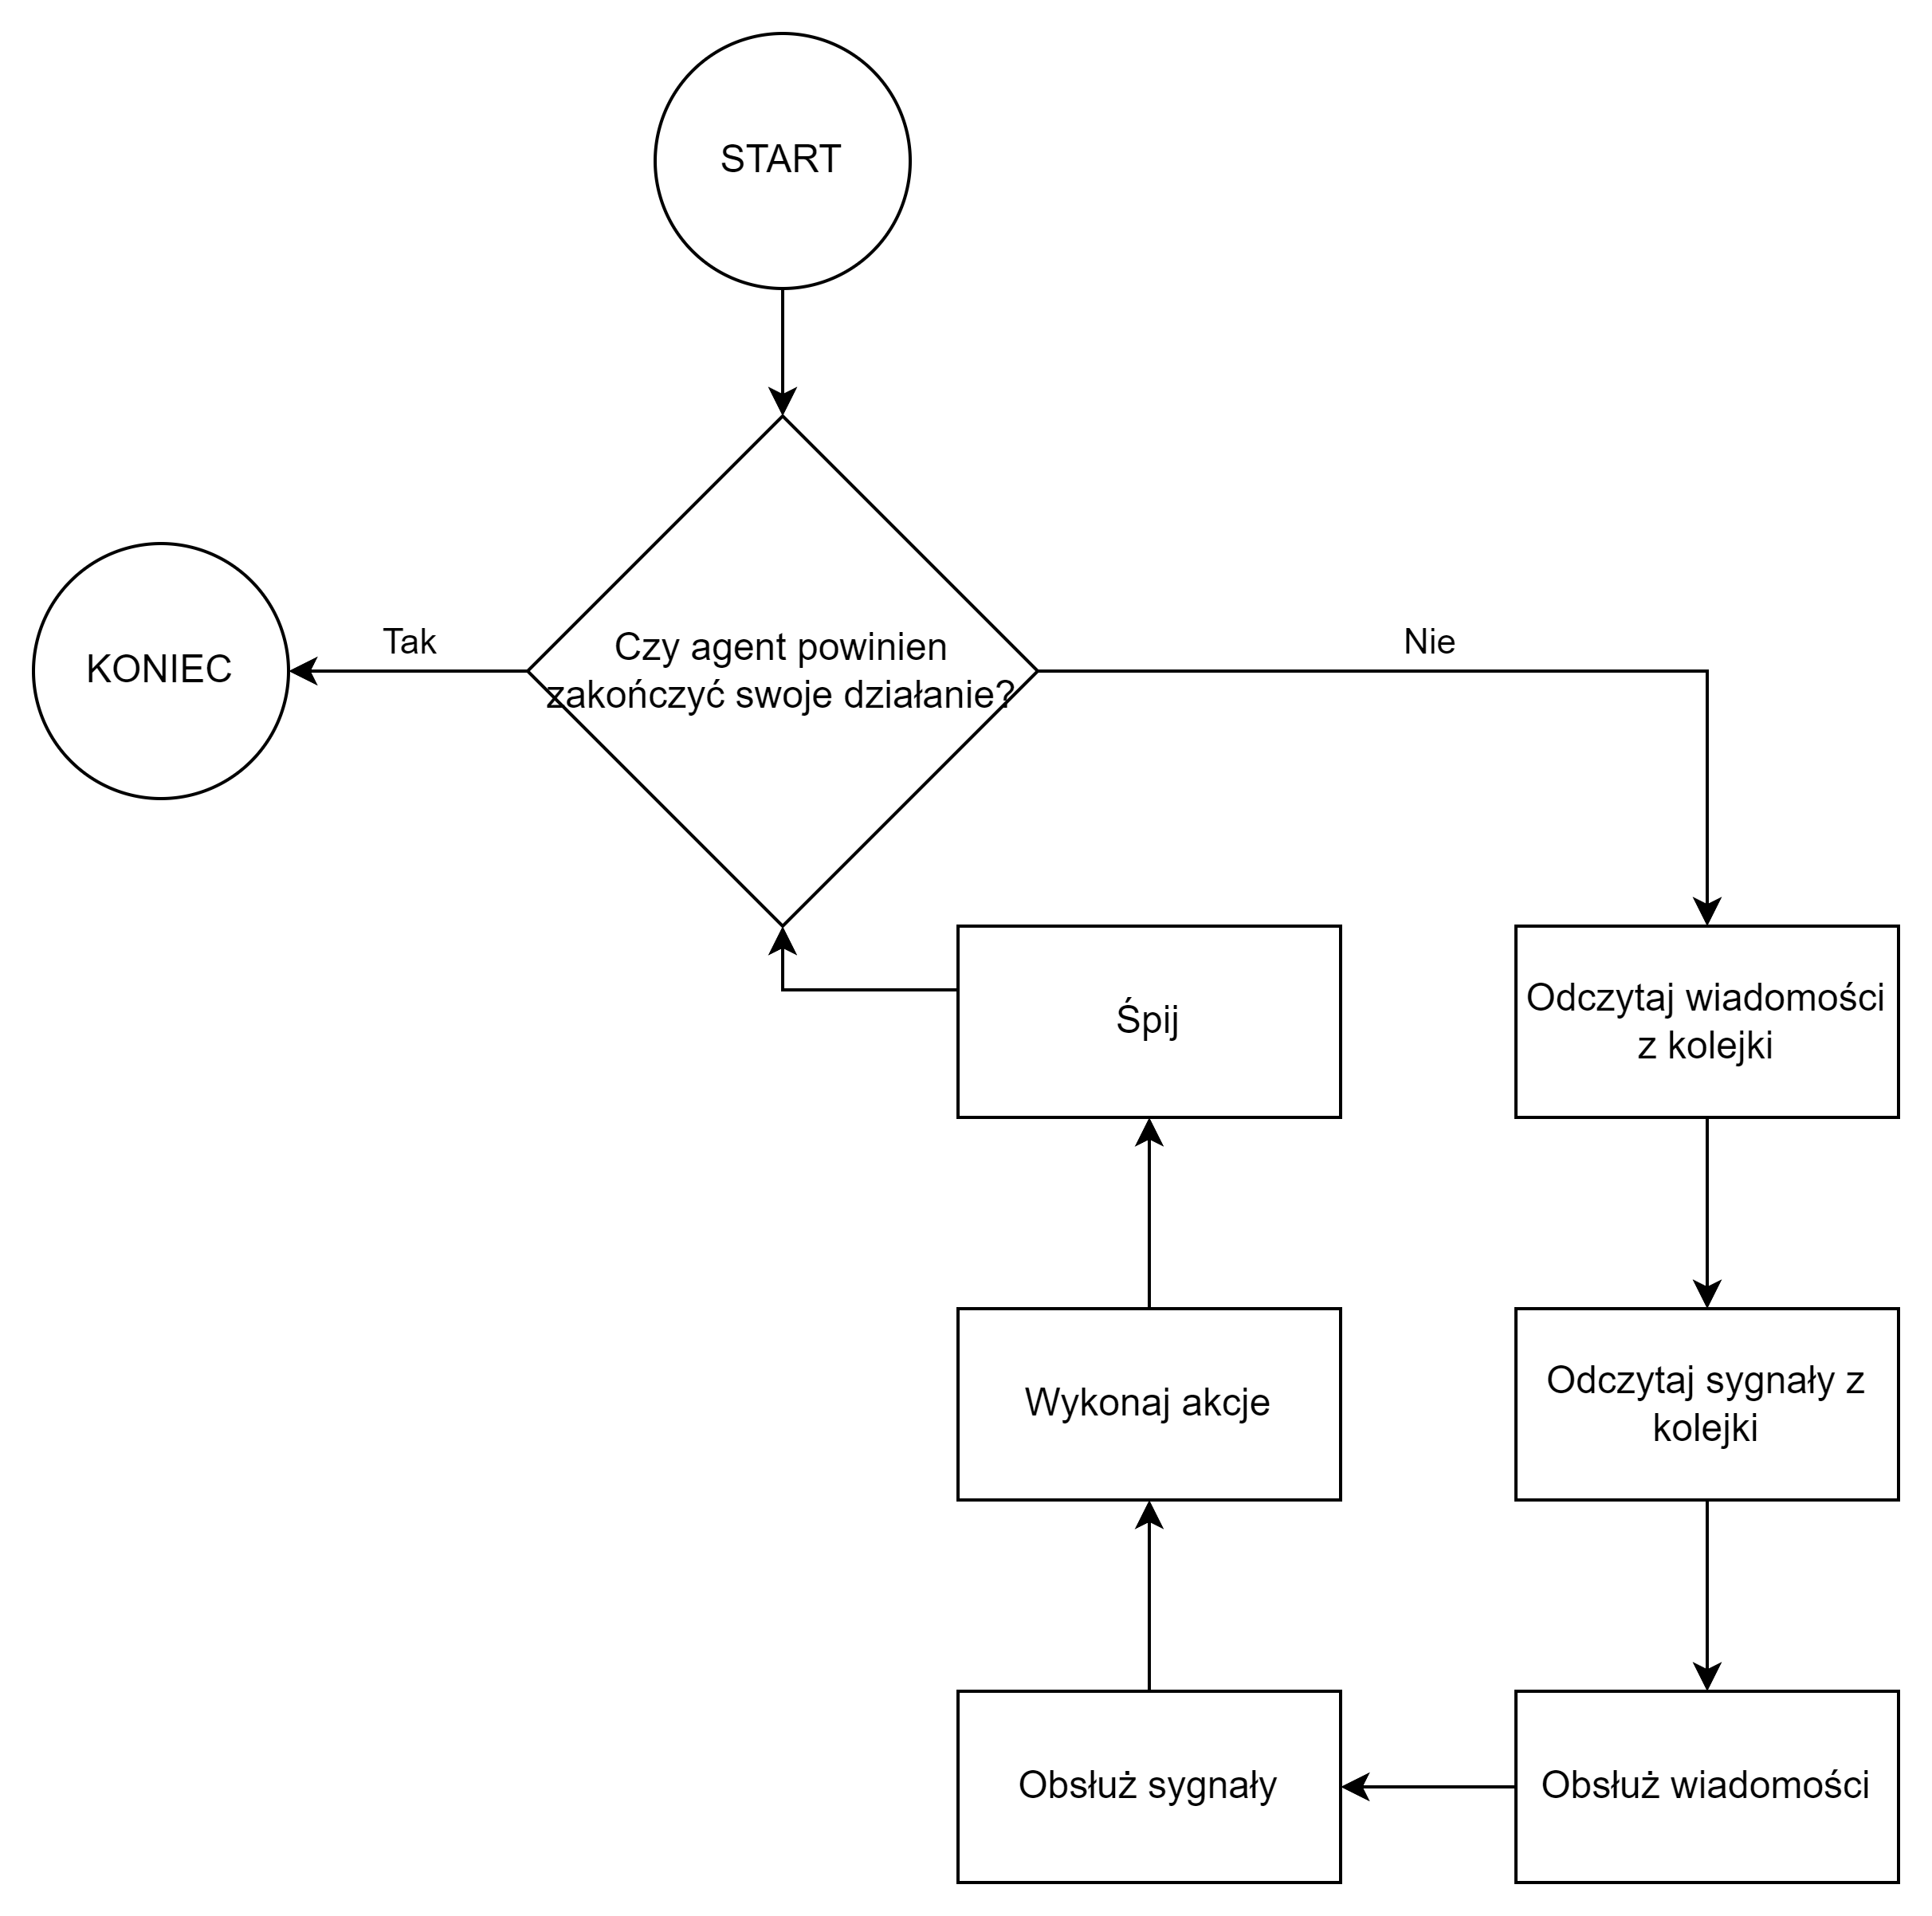
\includegraphics[width=\linewidth]{Agents - Agent Cycle}
    \caption{Cykl działania agenta}
    \label{fig:agentsAgentCycle}
    \source{Opracowanie Własne}
\end{figure}

\par Aby spełnić założenia systemu, ważnym było dokładne określenie wymiany wiadomości między agentami. Tabela \ref{tab:agentsMessagesSenderReceiver} pokazuje relację między typem wiadomości, a jej odbiorcą i nadawcą.

\begin{table}
    \centering
    \begin{tabular}{|c|c|c|} 
     \hline
     Rodzaj wiadomości & Nadawca & Odbiorca \\
     \hline
     \hline
     AskPositionMessage & Patrol Agent & Navigation Agent \\ 
     \hline
     CurrentLocationMessage & Navigation Agent & Patrol Agent \\ 
     \hline
     CurrentLocationMessage & Patrol Agent & HQ Agent \\ 
     \hline
     DestinationReachedMessage & Navigation Agent & Patrol Agent \\ 
     \hline
     GunFiredMessage & Gun Agent & Patrol Agent \\ 
     \hline
     GunFiredMessage & Patrol Agent & HQ Agent \\ 
     \hline
     IncidentInvestigationStartedMessage & Patrol Agent & HQ Agent \\ 
     \hline
     IncidentResolvedMessage & Patrol Agent & HQ Agent \\ 
     \hline
     JoinedShootingMessage & Patrol Agent & HQ Agent \\ 
     \hline
     NavigateToMessage & Patrol Agent & Navigation Agent \\ 
     \hline
     PatrolOfflineMessage & Patrol Agent & HQ Agent \\ 
     \hline
     PatrolOnlineMessage & Patrol Agent & HQ Agent \\ 
     \hline
     PatrolStatusChangedMessage & Patrol Agent & HQ Agent \\ 
     \hline
     ShowDistrictMessage & Patrol Agent & Navigation Agent \\ 
     \hline
     HandleIncidentOrderMessage & HQ Agent & Patrol Agent \\ 
     \hline
     PatrolDistrictOrderMessage & HQ Agent & Patrol Agent \\ 
     \hline
     SupportShootingOrderMessage & HQ Agent & Patrol Agent \\ 
     \hline
    \end{tabular}
    \caption{Tabela relacji wiadomości, nadawcy i odbiorcy}
    \label{tab:agentsMessagesSenderReceiver}
\end{table}

\par Zdefiniowane został również sygnały środowiskowe, służące agentom do obserwowania zmian w ich otoczeniu. Przedstawia je tabela \ref{tab:agentsEnvironmentSignals}.

\begin{table}
    \centering
    \begin{tabular}{|c|c|} 
     \hline
     Rodzaj sygnału & Agent \\
     \hline
     \hline
     DestinationReachedSignal & Navigation Agent \\ 
     \hline
     GunFiredSignal & Gun Agent \\ 
     \hline
     IncidentAlreadyOverSignal & Patrol Agent \\ 
     \hline
     IncidentResolvedSignal & Patrol Agent \\ 
     \hline
     PositionChangedSignal & Navigation Agent \\ 
     \hline
    \end{tabular}
    \caption{Tabela sygnałów środowiskowych wraz z ich odbiorcami}
    \label{tab:agentsEnvironmentSignals}
\end{table}

\par Aby komunikacja mogła nastąpić pomiędzy agentami, koniecznym jest ich odpowiednia konfiguracja. W szczególności dotyczy to patroli, które muszą wiedzieć, z jakich elementów się składają. W tym celu powstał interfejs \texttt{IPatrolInfoService}, który zapewnia informacje o identyfikatorach \emph{Patrol Agent}, \emph{Navigation Agent} i \emph{Gun Agent} oraz identyfikator patrolu, jako całości. Dokładniejszy opisz konfiguracji został omówiony w podrozdziale \ref{sec:konfiguracja}.